% Proposal converted into Latex format


\documentclass{article}
\usepackage{times}
\usepackage{graphicx}
\graphicspath{{./images/gg}} 

\begin{document}

% Article top matter
\title{e-Yantra Idea Competition 2019-20\\Team ID: 1082\\Automatic Khichadi Making and Vending Device} 
\maketitle

\section{Introduction/Motivation}
Many schools deliver mid-day meal facilities for children below 14 years. The intended scheme promises
qualitative and nutritious meals to the students. The idea is to provide a full packed energy meal to children
for well being. The Government is running this scheme successfully.\\
In recent years, it is observed that due
to human negligence while preparing the meal has resulted in poor quality as well as the occurrence of
catastrophic events. Even though the scheme is implemented, some constraints need to be put up for a better
quality of service.\\
The objective is to provide a smart automated system for the preparation of the meal. It
will result in less time consumption as well as help to monitor the quality of meal preparation thoroughly.
The system will help in monitoring hygiene in the kitchen and will make sure that the quality food of quality
standards will reach to students. The provided system is compatible with the electric supply and also
provided a solar facilitated battery. The implementation of the smart solution will help in ease of doing
business as well as will attain the goal for every school.

\section{Market Research/Literature Survey:}
The Mid-day Meal Scheme is a school meal program is organized by the Government of India. It is designed
for a better nutritional standard for children nationwide. It was started in the year of 2013. One of the
purposes is used to increase the attendance of students in government schools. The program provides a onetime meal for children below 14 years in government, government-aided schools. This scheme serves more
than 120,000,000 children all over 1,265,000 schools across the nation. Most of the children from rural areas
eat the meal provided by government agencies.\\
There are no parameters to show the hygiene of food being served to them. This sometimes results in poor
quality food service. One of the incidents has happened in Bihar where 23 children lost their lives after
eating their Mid Day meal on July 16, 2013. The MDMS guidelines indicate that the meal should be of good
quality, besides being nutritious, tasty, and easy to digest. The variation provided in the week menu keeps
the interest of the student. High standards of hygiene and cleanliness are expected to be maintained during
the cooking and serving of the meal.

\section{Hardware Requirements:}
\begin{itemize}
	\item Arduino MicroController
	\item Stepper Motor
	\item LCD
	\item Induction
	\item Power Supply
	\item Biometric Sensors
	\item DC Motors
	\item Storage Containers
	\item Pipes
	\item Stainless Steel Containers
	\item Slider
	\item Aluminium Body
\end{itemize}

\section{Software Requirements:}
\begin{itemize}
	\item Arduino IDE
\end{itemize}

\section{Implementation:}
The fingerprint of a student will be scanned through biometric. It verifies the parameters instructed in a
system in accordance with the fixed amount. The decided amount of Khichadi gets cooked in the processing
unit. The control panel rapidly activates the induction. When the bowl container is placed on induction, the
water flow sensor activates and a particular amount of water is released in bowl container and it starts
boiling. After measuring suitable temperature the sensors get to activate and they release the ingredients with
decided proportion. One by one, the ingredients are released in the boiled water in a specific proportion
already instructed to the sensor and motors are controlled by Arduino Uno. Onwards after few minutes of
delay, the decided quantity of rice is released and it allows for minutes of cooking. After that, the cooked
khichadi will be served to the candidate. \\

\begin{center}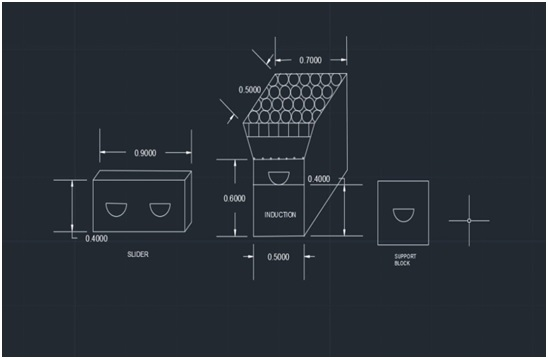
\includegraphics[scale=0.6]{schematic}\end{center}
\begin{center}Fig.1 Schematic Diagram of Automatic Khichadi Making and Vending Device\end{center}\\
This system is broadly divided into processing units and distribution unit:\\
\subsection{User Interface:}
The biometric sensor will take the fingerprint of the student. It will match the finger print
entered with that in the database and if a unique match is found, then the decided amount of Khichadi will be
served to the respective candidate. It initiates the response to the induction device to work and also
stimulates the slider for shifting the bowls in a row. Bio metric sensor helps in verification and also it will
take the records on a daily basis daily for government officials and save in the database.
\subsection{Ingredient Selection:}
Various sensors including water flow sensor and temperature sensor communicate
together and with specified delay to the stepper motor, they release the ingredients in the specified amount
instructed to the system. The sequence of delays is provided in the system according to processing.
Ingredients are selected as per the instructions and amount of food.
\subsection{Processing and Distribution Unit:}
A particular time period is set for cooking the food after mixing the
ingredients. When the food is cooked, it indicates the control panel. It indicates and displays that the food is
ready to serve. The distribution system gets stimulated. It consists of a slider and a couple of bowls that are
placed in the row. One by one bowls shifts towards the processing unit, the quantity set by the system is
served in each bowl. The block diagram of the proposed device is as follows:

\begin{center}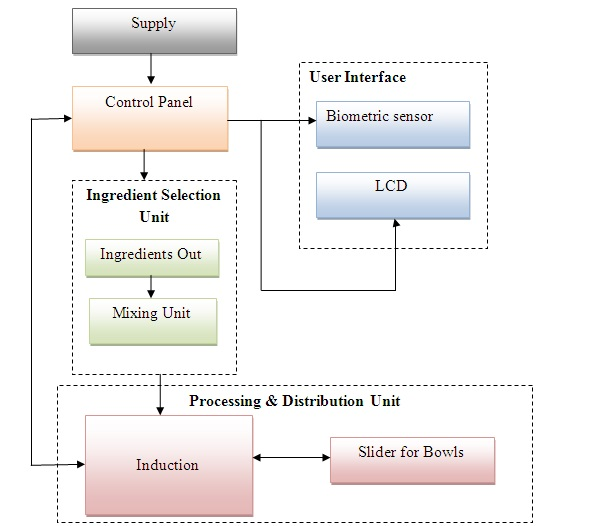
\includegraphics[scale=0.8]{block1082}\end{center}
\begin{center}Fig.2 Block Diagram of Automatic Khichadi Making and Vending Device\end{center}
\begin{center}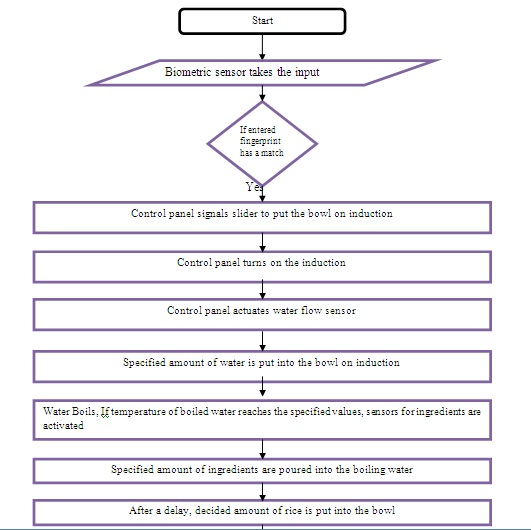
\includegraphics[scale=0.8]{flow1}\end{center}
\begin{center}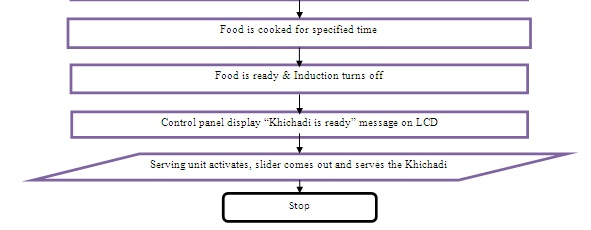
\includegraphics[scale=0.8]{flow2}\end{center}
\begin{center}Fig.2 Flow Diagram of Automatic Khichadi Making and Vending Device\end{center}

\section{Feasibility}
The existing system of khichadi making process takes huge manpower, though it is a more time-consuming
process. There are no parameters available for monitoring each phase of process. Examination of sanitation
while cooking is a necessity. To automate this entire process, and provide a more efficient optimal solution,
we have proposed the idea of automatic khichadi making and vending devices.\\
Due to automation applied
the probability of time-saving increased with good efficiency and nutrition standard maintained. Limitations
like a huge quantity of food cooking in less time, huge manpower and processing cost are dealt with by the
system. Transformation of existing systems dependent on manpower to the automated system leads to
efficiency, providing nutritious food maintenance having the advantage of less time consumption and a
healthy living environment.
\begin{thebibliography}{9}
	\bibitem{}
	 https://www.britannica.com/topic/vending-machine
	 
	 \bibitem{}
	Mid-day Meal Scheme
	https://en.wikipedia.org/wiki/Midday\textunderscore Meal\textunderscore Scheme?wprov=sfla1
	 
	 \bibitem{}
	https://www.mouser.in/Sensors/Flow-Sensors/\textunderscore /N-            
	zqi2?gclid=Cj0KCQiAno\textunderscore uBRC1ARIsAB496IWJ6SUidpV4XQebI90Eyus\textunderscore uR\textunderscore rJpTio8QTyqESkpekAV0lMC6otX
	 
	\bibitem{}
 https://www.electronicshub.org/types-of-biometric-sensors/
 
    \bibitem{}
    https://www.cda.eu/hobs/how-does-induction-cooking-work/
\end{thebibliography} %Must end the environment

\end{document}  %End of document.